\documentclass[12pt]{article}

\usepackage{parskip,amsthm,amsmath,amsfonts,amssymb}
\usepackage{multicol,cancel}
\usepackage[shortlabels]{enumitem}
\usepackage[letterpaper,margin=1in,bottom=0.7in]{geometry}
\newcommand{\dd}[2]{\dfrac{d #1}{d #2}}
\newcommand{\ddd}[2]{\dfrac{d^2 #1}{d #2^2}}
\newcommand{\pd}[2]{\dfrac{\partial #1}{\partial #2}}
\newcommand{\ppd}[2]{\dfrac{\partial^2 #1}{\partial #2^2}}
\newcommand{\ppdd}[3]{\dfrac{\partial^2 #1}{\partial #2\partial #3}}
\newcommand{\brf}[2]{\left(\frac{#1}{#2}\right)}
                       % Bracket-frac, e.g. for (n\pi x/L) in Fourier series
\newcommand{\fsin}[1]{\sin\brf{#1 \pi x}{L}}
\newcommand{\fcos}[1]{\cos\brf{#1 \pi x}{L}}
\newcommand{\fsint}[1]{\sin\brf{#1 \pi t}{L}}
\newcommand{\fcost}[1]{\cos\brf{#1 \pi t}{L}}
\newcommand{\RR}{\mathbf{R}}
\newcommand{\CC}{\mathbf{C}}
\newcommand{\ZZ}{\mathbf{Z}}
\newcommand{\mks}[1]{\begin{flushright}(#1 marks)\end{flushright}}

\usepackage{tikz}
\newcommand{\lapl}[6]{
\begin{tikzpicture}[scale=2]
  \draw (0,0) -- (0,1);
  \draw (0,1) -- (1,1);
  \draw (1,1) -- (1,0);
  \draw (1,0) -- (0,0);
  \node at (0.5,0.5) {$#6$};
  \node [below] at (0.5,0) {$#1(x,0)=#2$};
  \node [above] at (0.5,1) {$#1(x,\pi)=#3$};
  \node [left] at (0,0.5) {$#1(0,y)=#4$};
  \node [right] at (1,0.5) {$#1(\pi,y)=#5$};
\end{tikzpicture}
}

\newcommand{\onelapl}[6]{
\begin{tikzpicture}[scale=2]
  \draw (0,0) -- (0,1);
  \draw (0,1) -- (1,1);
  \draw (1,1) -- (1,0);
  \draw (1,0) -- (0,0);
  \node at (0.5,0.5) {#6};
  \node [below] at (0.5,0) {$#1(x,0)=#2$};
  \node [above] at (0.5,1) {$#1(x,1)=#3$};
  \node [left] at (0,0.5) {$#1(0,y)=#4$};
  \node [right] at (1,0.5) {$#1(1,y)=#5$};
\end{tikzpicture}
}


\newcommand{\mlapl}[6]{
\begin{tikzpicture}[scale=2]
  \draw (0,0) -- (0,1);
  \draw (0,1) -- (1,1);
  \draw (1,1) -- (1,0);
  \draw (1,0) -- (0,0);
  \node at (0.5,0.5) {#1};
  \node [below] at (0.5,0) {$#6(x,0)=#2$};
  \node [above] at (0.5,1) {$#6(x,\pi)=#3$};
  \node [left] at (0,0.5) {$#6(0,y)=#4$};
  \node [right] at (1,0.5) {$#6(\pi,y)=#5$};
\end{tikzpicture}
}
\newcommand{\laplneu}[6]{
\begin{tikzpicture}[scale=2]
  \draw (0,0) -- (0,1);
  \draw (0,1) -- (1,1);
  \draw (1,1) -- (1,0);
  \draw (1,0) -- (0,0);
  \node at (0.5,0.5) {#6};
  \node [below] at (0.5,0) {$#1(x,0)=#2$};
  \node [above] at (0.5,1) {$#1(x,\pi)=#3$};
  \node [left] at (0,0.5) {$\partial_x#1(0,y)=#4$};
  \node [right] at (1,0.5) {$\partial_x#1(\pi,y)=#5$};
\end{tikzpicture}
}

\theoremstyle{remark}
\newtheorem{rmk}{Remark}

\theoremstyle{definition}
\newtheorem{question}{Question}
\newtheorem{answer}{Answer}


%%%%%%%%%%%%%%%%%% Add extra space before theorems

\begingroup 
\makeatletter 
\@for\theoremstyle:=definition,remark,plain,TheoremNum\do{% 
\expandafter\g@addto@macro\csname th@\theoremstyle\endcsname{% 
\addtolength\thm@preskip\parskip 
}% 
} 
\endgroup 

\title{Methods 3 - Question Sheet 1}
\author{J. Evans}
\date{}

\begin{document}
\maketitle

\begin{question}(4 marks)\\
Let $m,n$ be positive integers. Verify the integral identities:
\[
\frac{1}{L}\int_{-L}^L\fcos{n}\fcos{m}dx=\delta_{mn}
\]
and
\[
\frac{1}{L}\int_{-L}^L\fcos{n}\fsin{m}dx= 0.
\]
\end{question}

\begin{answer}
In the first case we have $\frac{1}{L}\fcos{n}\fcos{m}=\frac{1}{2L}\left(\fcos{(n+m)}+\fcos{(n-m)}\right)$ and since $\int_{-L}^L\fcos{N}dx=0$ unless $N=0$ the integral of $\frac{1}{L}\fcos{n}\fcos{m}$ vanishes unless $n=m$, in which case it becomes $\frac{1}{2L}\int_{-L}^Ldx=1$ as required.\mks{2}

In the second case we have $\frac{1}{L}\fcos{n}\fsin{m}=\frac{1}{2L}\left(\fsin{(m+n)}+\fsin{(m-n)}\right)$ and since $\int_{-L}^L\fsin{N}dx=0$ the integral of $\frac{1}{L}\fcos{n}\fsin{m}$ vanishes as required.\mks{2}
\end{answer}

\newpage

\vspace{0.5cm}

\begin{question}(10 marks for * parts)\\
For each of the following functions, find its half-range sine series on $[0,\pi]$:
\begin{enumerate}[(a)]
\item * $f(x)=x^3-\pi^2x$.
\item * $f(x)=\cos x+\dfrac{2x}{\pi}-1$.
\item $f(x)=e^x-\dfrac{(e^{\pi}-1)x}{\pi}-1$.
\item $f(x)=\begin{cases}x&\mbox{ if }x\in\left[0,\tfrac{\pi}{2}\right]\\ \pi-x&\mbox{ if }x\in\left[\tfrac{\pi}{2},\pi\right].\end{cases}$
\item $f(x)=\sin x$.
\end{enumerate}
\end{question}

\begin{answer}
In each case the Fourier coefficient $b_n$ is given by $\frac{2}{\pi}\int_0^{\pi}f(x)\sin(nx)dx$.
\begin{enumerate}
\item[(a)] Integrating by parts we get
\begin{align*}
\frac{2}{\pi}\int_0^{\pi}(x^3-\pi^2x)\sin(nx)dx&=\frac{2}{\pi}\left(\cancelto{0}{\left[-(x^3-\pi^2x)\frac{\cos(nx)}{n}\right]_0^{\pi}}+\frac{1}{n}\int_0^{\pi}(3x^2-\pi^2)\cos(nx)dx\right)\\
&=\frac{2}{n\pi}\left(\cancelto{0}{\left[(3x^2-\pi^2)\frac{\sin(nx)}{n}\right]_0^{\pi}}-\frac{1}{n}\int_0^{\pi}6x\sin(nx)\right)\\
&=-\frac{2}{n^2\pi}\left(\left[-6x\frac{\cos(nx)}{n}\right]_0^{\pi}+\frac{1}{n}\int_0^{\pi}6\cos(nx)dx\right)\\
&=\frac{12}{n^3\pi}(\pi(-1)^{n})-\cancelto{0}{\frac{12}{n^4\pi}\left[\sin(nx)\right]_0^{\pi}}\\
&=\frac{12(-1)^{n}}{n^3}.
\end{align*}
\mks{5}
\item[(b)] We need to find $\frac{2}{\pi}\int_0^{\pi}\left(\cos x+\frac{2x}{\pi}-1\right)\sin(nx)dx$. The cosine integral gives
\begin{align*}
\frac{2}{\pi}\int_0^{\pi}\cos x\sin(nx)dx&=\frac{1}{\pi}\int_0^{\pi}\left(\sin(n+1)x+\sin(n-1)x\right)dx\\
&=-\frac{1}{\pi}\left(\frac{(-1)^{n+1}}{n+1}+\frac{(-1)^{n-1}}{n-1}-\frac{1}{n+1}-\frac{1}{n-1}\right)\\
&=\frac{2n(1+(-1)^n)}{\pi(n^2-1)}
\end{align*}
\mks{2}
(note that we should treat $n=1$ separately as we divide by $n-1$; the integral becomes $(1/\pi)\int_0^{\pi}(\sin(2x)+\sin(0x))dx=0$).

The $2x/\pi$ term gives
\begin{align*}
\frac{4}{\pi^2}\int_0^{\pi}x\sin(nx)dx&=\frac{4}{\pi^2}\left(\left[-x\frac{\cos(nx)}{n}\right]_0^{\pi}+\frac{1}{n}\int_0^{\pi}\cos(nx)dx\right)\\
&=-\frac{2}{\pi}\left(\frac{2(-1)^n}{n}\right)+\cancelto{0}{\frac{4}{n^2\pi^2}\left[\sin(nx)\right]_0^{\pi}}
\end{align*}
\mks{2}
and the constant term gives
\[\frac{2}{\pi}\int_0^{\pi}(-1)\sin(nx)dx=\frac{2((-1)^n-1)}{n\pi}\]
\mks{1}
so in total we have
\begin{align*}
b_n&=\frac{2}{\pi}\left(\frac{n(1+(-1)^n)}{n^2-1}-\frac{2(-1)^n}{n}+\frac{(-1)^n-1}{n}\right)\\
   &=\frac{2}{\pi}((-1)^n+1)\left(\frac{n}{n^2-1}-\frac{1}{n}\right)\\
   &=\frac{2((-1)^n+1)}{\pi n(n^2-1)}
\end{align*}
(and $b_1=0$).
\item[(c)] $b_n=\frac{2(e^{\pi}(-1)^n-1)}{n\pi(n^2+1)}$.
\item[(d)] $b_n=\frac{4\sin(n\pi/2)}{n^2\pi}$.
\item[(e)] $b_1=1$, $b_n=0$ for $n>1$.
\end{enumerate}
\end{answer}
\newpage

\vspace{0.5cm}

\begin{question}(6 marks)\\
\begin{enumerate}
\item[(a)] Suppose that $F(x)$ is an odd function on $[-\pi,\pi]$. Prove that $\int_{-\pi}^{\pi}F(x)^2dx=2\int_0^{\pi}F(x)^2dx$.
\end{enumerate}
Consider the odd function $F(x)$ on $[-\pi,\pi]$ equal to $x(\pi-x)$ on $[0,\pi]$. The Fourier series of $F$ was found in lectures:
\[F(x)=\frac{8}{\pi}\sum_{n\mbox{ odd}}\frac{\sin(nx)}{n^3}.\]
\begin{enumerate}
\item[(b)] Use this to show that
\[T:=\frac{1}{1^6}+\frac{1}{3^6}+\frac{1}{5^6}+\cdots=\frac{\pi^6}{960}.\]
\item[(c)] Deduce that if
\[S:=\frac{1}{1^6}+\frac{1}{2^6}+\frac{1}{3^6}+\cdots\]
then $S=T+\frac{S}{64}$ and hence calculate $S$.
\end{enumerate}
\end{question}


\begin{answer}
\begin{enumerate}
\item[(a)] $\int_{-\pi}^{\pi}F(x)^2dx=\left(\int_{-\pi}^0+\int_0^{\pi}\right)F(x)^2dx$. Changing variables $x\to u=-x$ in the first integral gives $\int_{\pi}^0F(-u)^2(-du)=\int_0^{\pi}(-F(u))^2du=\int_0^{\pi}F(x)^2dx$ hence $\int_{-\pi}^{\pi}F(x)^2dx=2\int_0^{\pi}F(x)^2dx$.
\mks{1}
\item[(b)] Parseval's theorem gives
\[\frac{64}{\pi^2}\sum_{n\mbox{ odd}}\frac{1}{n^6}=\frac{1}{\pi}\int_{-\pi}^{\pi}F(x)^2dx=\frac{1}{\pi}\int_0^{\pi}x^2(\pi-x)^2dx\]
by part (a). This integral is
\begin{align*}
\frac{2}{\pi}\int_0^{\pi}(x^2\pi^2-2x^3\pi+x^4)dx&=\frac{2}{\pi}\left[\frac{x^3\pi^2}{3}-2\frac{x^4\pi}{4}+\frac{x^5}{5}\right]_{x=0}^{\pi}\\
&=2\pi^4\left(\frac{1}{3}-\frac{1}{2}+\frac{1}{5}\right)\\
&=\frac{\pi^4}{15}.
\end{align*}
\mks{2}
Thus
\[\sum_{n\mbox{ odd}}\frac{1}{n^6}=\frac{\pi^6}{15\times 64}=\frac{\pi^6}{960}\]
as required.\mks{1}
\item[(c)] We have $S=\sum_{n\mbox{ odd}}\frac{1}{n^6}+\sum_{n\mbox{ even}}\frac{1}{n^6}=T+\sum_n\frac{1}{(2n)^6}=T+\frac{S}{64}$. Therefore $S(1-1/64)=63S/64=T=\pi^6/(15\times 64)$ so $S=\pi^6/(15\times 63)$ or
\[\sum_{n=1}^{\infty}\frac{1}{n^6}=\frac{\pi^6}{945}.\]
\mks{2}
\end{enumerate}
\end{answer}
\newpage

\vspace{0.5cm}

\begin{question}\ \\
Find the half-range cosine series of $f(x)=x^4-2\pi^2x^2$ on $[0,\pi]$. By considering $f(0)$, show that
\[\sum_{n=1}^{\infty}\frac{(-1)^{n+1}}{n^4}=\frac{7\pi^4}{720}\]
\end{question}

\begin{answer}
$a_0=-\frac{14\pi^4}{15}$, $a_n=\frac{48(-1)^{n+1}}{n^4}$ so
\[f(x)=-\frac{7\pi^4}{15}+48\sum_{n=1}^{\infty}\frac{(-1)^{n+1}}{n^4}\cos(nx).\]
Setting $x=0$ gives $f(0)=0$ and
\[\sum_{n=1}^{\infty}\frac{(-1)^{n+1}}{n^4}=\frac{7\pi^4}{48\times 15}=\frac{7\pi^4}{720}.\]
\end{answer}
\newpage

\vspace{0.5cm}

\begin{question}\ \\
Imagine there were a function $\delta(x)$ with the property that
\[\int_{-1}^1\delta(x)g(x)dx=g(0)\]
for any function $g$. What would the Fourier series of $\delta$ be? What might the graph of the function $\delta$ look like? Let $\delta_N$ denote the approximation to $\delta$ obtained by summing the first $N$ terms of its Fourier series. Show that $\delta_N(x)=\frac{\sin((N+1/2)\pi x)}{2\sin(\pi x/2)}$. Use a computer to plot $\delta_N$ for some small values of $N$. As $N$ increases, does the plot start to look like the graph you imagined?

{\em $\delta$ is called the Dirac delta function; it is not really a function, but fits into the theory of ``distributions''. The sequence of truncations is called the Dirichlet kernel; analysis of the integral $\int\delta_N(x)F(x+y)dx$ is involved in proving that the Fourier series of $F$ converges in the $L^2$-sense to $F$.}
\end{question}


\begin{answer}
We would have
\[\int_{-1}^1\delta(x)\sin(n\pi x)dx=\sin(n\pi 0)=0\]
and
\[\int_{-1}^1\delta(x)\cos(n\pi x)dx=\cos(n\pi 0)=1\]
so
\[\delta(x)=\frac{1}{2}+\cos(\pi x)+\cos(2\pi x)+\cos(3\pi x)+\cdots\]
Here are plots of the first six truncations, gradually tending to an infinitely tall spike concentrated near 0.

\begin{center}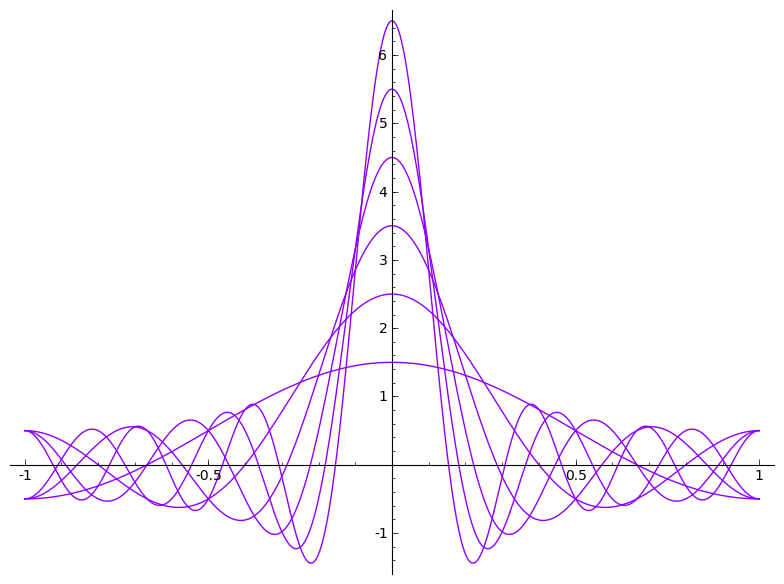
\includegraphics[width=300px]{delta-all.png}\end{center}

To see that $\delta_N(x)=\frac{\sin((N+1/2)\pi x)}{2\sin(\pi x/2)}$, note that
\[\sin(\pi x/2)\cos(n\pi x)=\frac{1}{2}(\sin((n+1/2)\pi x)-\sin((n-1/2)\pi x))\]
so there are many cancelling terms in the sum
\[\sin(\pi x/2)(\cos(\pi x)+\cos(2\pi x)+\cdots+\cos(N\pi x))\]
which simplifies to
\[\frac{1}{2}(\sin((N+1/2)\pi x)-\sin(\pi x/2))\]
Thus
\[\cos(\pi x)+\cos(2\pi x)+\cdots+\cos(N\pi x)=\frac{\sin((N+1/2)\pi x)}{2\sin(\pi x/2)}-\frac{1}{2}\]
as required.
\end{answer}
\end{document}
